\section{DESENVOLVIMENTO}

\lipsum[2] \\

\lipsum[3]

\subsection{TÍTULOS DE SESSÕES}

\subsubsection{Regras}

\begin{itemize} 
    \item Título primário: negrito e em letras maiúsculas;
    \item Título secundário: letras maiúsculas sem negrito;
    \item Título terciário: negrito e com iniciais em maiúsculas;
    \item Título quaternário: iniciais em maiúsculas e sem negrito;
    \item Título quinário: itálico e com iniciais em maiúsculas;
    \item Título sem indicativos numéricos: Caixa alta, negrito, centralizado;
\end{itemize}

Títulos que ocupem mais de uma linha devem ser, a partir da segunda linha, alinhados abaixo da primeira letra da primeira palavra do título.

\newpage

\subsection{SUMÁRIO}

\subsubsection{Exemplo}

\begin{figure}[h]
    \centering
    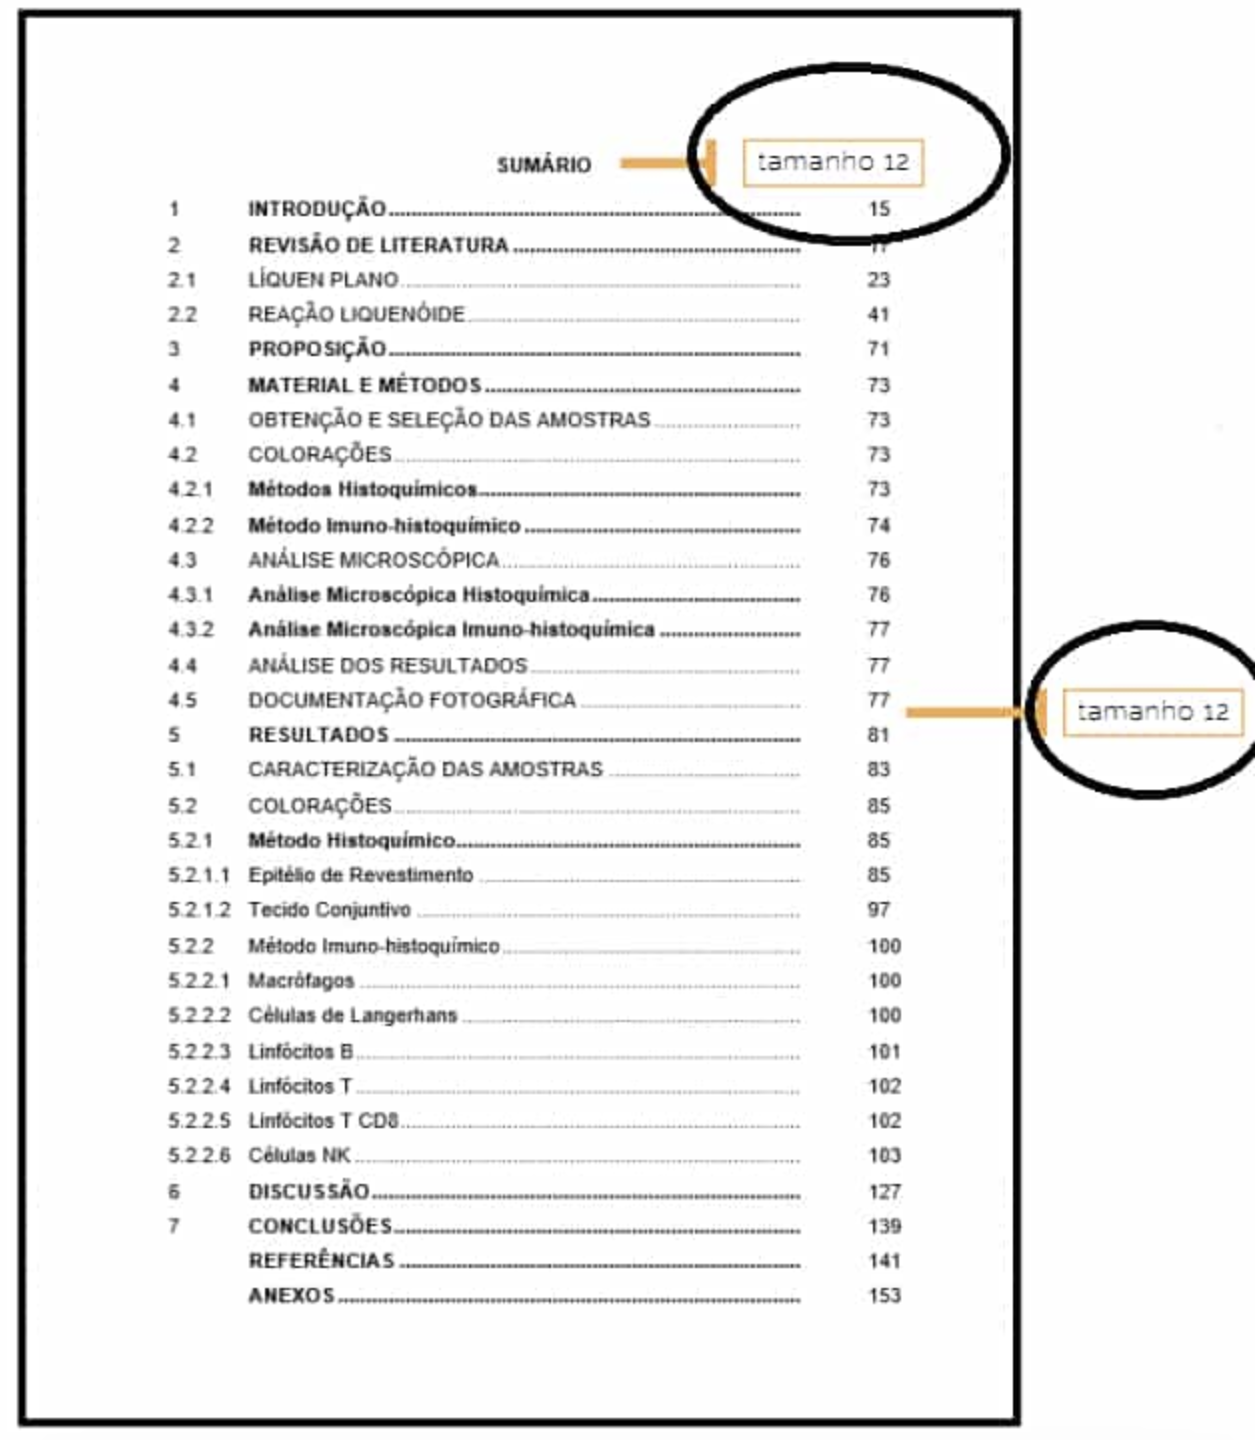
\includegraphics[width=0.9\textwidth]{Figuras/exemplo_sumario.png} % Change to the path of your image
    \caption{Exemplo de um sumário.}
    \label{fig:exemplo_sumario}
\end{figure}

\newpage

\subsubsection{Regras}

\begin{itemize}
    \item A margem superior e esquerda deverá ser de 3 cm;
    \item A margem inferior e direita deverá ser de 2 cm;
    \item O título deverá ficar centralizado e em letra maiúscula;
    \item O sumário deverá ficar antes da introdução;
    \item Você deverá organizar de acordo com os capítulos, seções e partes, tudo na ordem que seu trabalho será!
    \item O sumário deverá ficar depois da capa, folha de rosto, folha de aprovação, dedicatória, resumo ou listas;
    \item A palavra “sumário” ficará no topo da página em negrito, com a mesma fonte e tamanho do resto do texto;
    \item O espaçamento entre as linhas deverá ser de 1,5;
    \item O tamanho da fonte deverá ser 12;
    \item Não deverão conter outros textos, apenas os títulos das divisões e subdivisões;
    \item Os capítulos devem ser escritos com todas as letras em caixa alta, com fonte tamanho 12, em negrito e em alinhamento à esquerda;
    \item Os subcapítulos devem ter a mesma formatação dos capítulos, mas com apenas a primeira letra maiúscula, o resto em letra minúscula;
    \item Os subcapítulos não são em negrito como os capítulos.
\end{itemize}

\newpage

\subsection{MATEMÁTICA}

You can use mathematical formatting, such as:
\[
f(x) = \int_{0}^{\infty} e^{-x^2} \, dx
\]
or numbered equations like:
\begin{equation}
    E = mc^2
\end{equation}

\subsection{FAZENDO REFERENCIAS BIBLIOGRÁFICAS}

% Para fazer referencias bibliograficas em LaTex, voce deve usar o comando \cite{dirac} para fazer uma citação à algum artigo mencionado no arquivo \texttt{Referencias.bib}.

% \cite{website:ArduinoLabview}
% \cite{website:OPENSOURCESW}
% \cite{website:OPENSOURCEHW}
